
En la siguiente aparatado intentaremos validar dos hipótesis: que el modelo generado realmente puede ser identificado como un hablante extranjero de habla inglesa y al mismo tiempo que este posee un grado de inteligibilidad aceptable.

Para eso se condujo una encuesta perceptual donde, dado un participante, se le presentó un audio con una oración semánticamente impredecible, fonéticamente balanceada y con distintos grados de mezcla de español e ingles, se le pidió que la transcribiera y que intentara identificar la nacionalidad del mismo.

Para la experimentación, se generaron diez oraciones distintas variando el nivel de mezcla de los modelos generados entre $30\%$ de ingles - $70\%$ castellano hasta $70\%$ de ingles - $30\%$ de castellano.

Los utternaces utilizados fueron generados de manera algorítmica tomando palabras de manera aleatoria de una lista de sustantivos, adjetivos y verbos y realizando correcciones donde fuera necesario para mantener el balanceo fonético.

\begin{enumerate}
\item Utternace 1: Mi montaña aguileña recorrió la esquina
\item Utternace 2: Aquel fuerte vidrio prefirió aquel botón
\item Utternace 3: Este enjoyado juez comprará nuestro corchete
\item Utternace 4: Tu estrecho posavasos gritó la fechoría
\item Utternace 5: Nuestro nublado tigre concluyó a este chupetín
\item Utternace 6: Su profundo riñón apoyó a Julio
\item Utternace 7: El frío churrasco oyó lo de Polonia
\item Utternace 8: Las acongojadas cotorras sonrieron a mi círculo
\item Utternace 9: Ese gruñón perro prometió a esos cuñados
\item Utternace 10: El nudillo Argentino perdió su vaso
\end{enumerate}


La encuesta se realizó a través de internet, con el mismo set de instrucciones para todos los participantes y pidiendo como requerimiento la utilización de auriculares. Cada participante podía contestar un máximo $5$ veces (otorgándoles siempre audios distintos).

La misma se llevó a cavo desde el $18$ de octubre de $2017$ hasta el primero de diciembre del mismo año, tiempo durante el cual fue publicada en distintas redes sociales y listas de emails de la facultad.

\subsection{Interface}

A continuación se presenta la interfase que utilizamos para realizar la encuesta junto con las decisiones de diseño que fueron tomadas a lo largo de la misma. 

Al entrar en la pagina de la encuesta todos los participantes fueron presentados con la siguiente pantalla principal:

\begin{center}
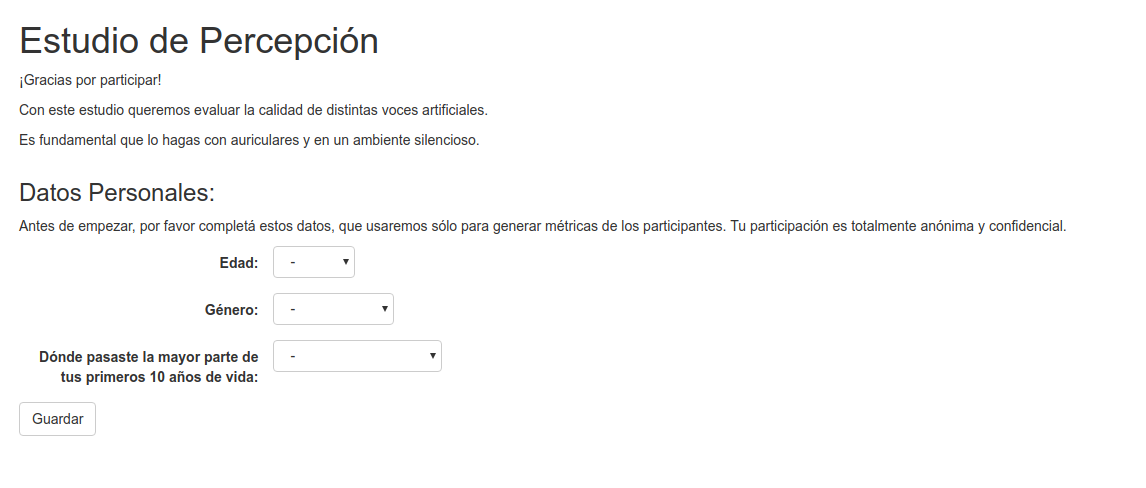
\includegraphics[scale=0.4]{estudio_online/estudio1.png}
\end{center}

Con el objetivo de no influir el las respuestas de los participantes participantes, se procuró darles a los participantes la información indispensable para completar la encuesta. En ningún momento se especifica que buscábamos con este estudio.

Con la intención de que los resultados fueran lo menos variables posibles, se le pidió a cada participante que realizara la encuesta con auriculares y en un lugar silencioso.

Además, le pedimos a cada participante que indique su genero, su edad y la provincia en la que transcurrido la mayor parte de su infancia.

Una vez que completados estos datos, se les presentaba otra vista con las instrucciones especificas para completar la encuesta:

\begin{center}
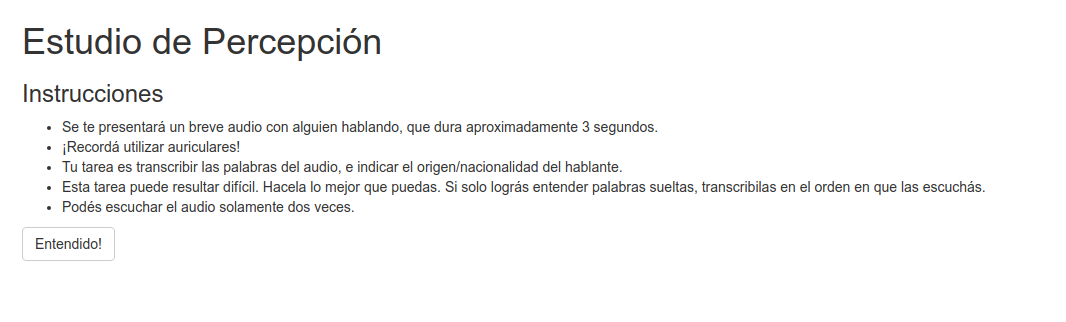
\includegraphics[scale=0.4]{estudio_online/estudio2.png}
\end{center}

Una vez presionado el botón de ``entendido!'' se les presentaba un audio, que podían escuchar un máximo de $2$ veces, una caja de texto libre donde plasmar la transcripción del mismo y una caja de texto libre donde podían escribir la nacionalidad correspondiente a la voz.

\begin{center}
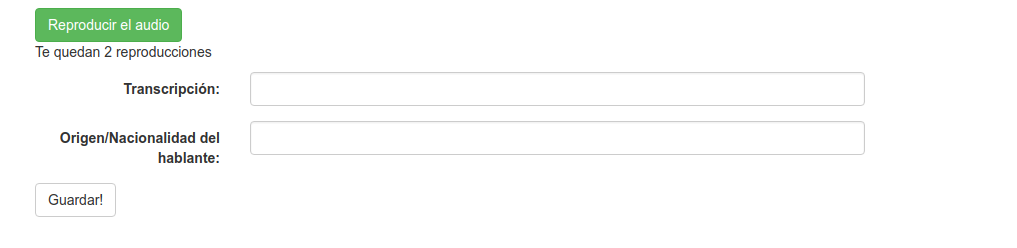
\includegraphics[scale=0.4]{estudio_online/estudio3.png}
\end{center}

Una vez que la respuesta era guardada, si el participante todavía no había contestado 5 veces, se le preguntaba si quería continuar transcribiendo otro audio, o de caso contrario se le presentaba un mensaje donde se le indicaba que ya podía cerrar la encuesta.

\pagebreak

\subsection{Resultados}

A modo de introducción, comenzaremos mostrando los datos demográficos de los participantes. Continuaremos con un análisis mas exhaustivo de la inteligibilidad y por otro lado de la nacionalidad atribuida. Por ultimo para contestar compondremos estos dos ejes para intentar contestar la hipótesis original.

\subsubsection{Datos demográficos}

Se encuestaron $109$ participantes de los cuales se obtuvieron $352$ resultados.

Del total de participantes, $49$ pertenecían al rango comprendido entre $18$ y $25$ años, $43$ estaban en el rango $26$-$35$. $17$ de los participantes eran mayores a $35$ años:  

\begin{figure}[htp]
\begin{center}
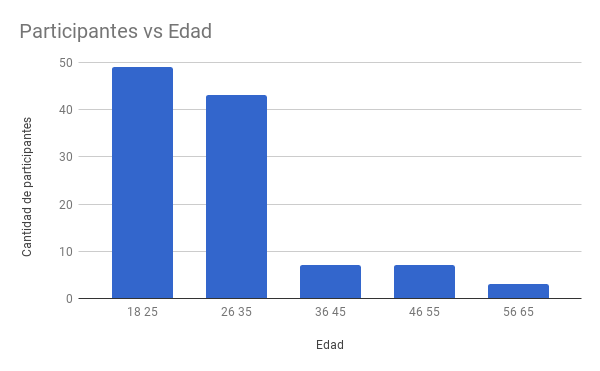
\includegraphics[scale=0.3]{datosDemograficos/edad.png}
\end{center}
\caption{Edad de los participantes}
\label{pics:blablabla}
\end{figure}


Con respecto al genero de los participantes, $187$ respuestas fueron brindadas por participantes del genero femenino mientras que $163$respuestas fueron brindadas por participante del genero masculino.


\begin{figure}[htp]
\begin{center}
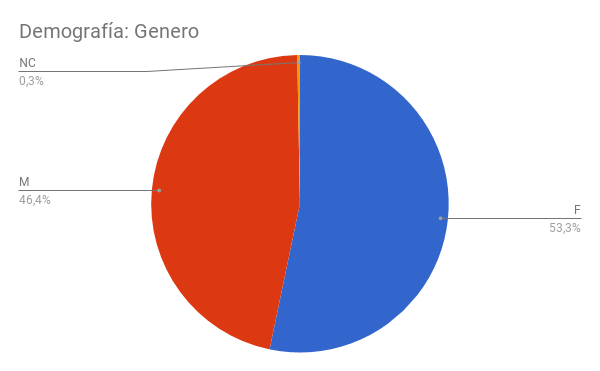
\includegraphics[scale=0.3]{datosDemograficos/genero.png}
\end{center}
\caption{Genero}
\label{pics:blablabla}
\end{figure}


En los datos referentes a la región en que cada participante pasó su infancia puede verse una predominancia de personas del Gran Buenos Aires con $45\%$, seguido por un $30\%$ que pasaron su infancia en la Capital Federal. Menos del $25\%$ pertenece al resto de las provincias Argentinas. Además, $10$ personas contestaron que se criaron fuera del país.


\begin{figure}[htp]
\begin{center}
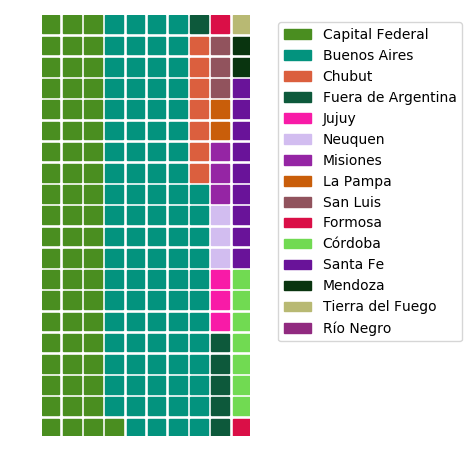
\includegraphics[scale=0.3]{datosDemograficos/infancia.png}
\end{center}
\caption{Distribución Territorial}
\label{pics:blablabla}
\end{figure}

\subsubsection{Inteligibilidad}

Para el análisis de resultados utilizaremos la distancia de Levenshtein con inserciones, remociones y reemplazos. Respetando los acentos pero sin tener en cuenta mayúsculas o minúsculas.

Presentamos aquí los resultados obtenidos sin ningún tipo de modificación:

\begin{figure}[htp]
\begin{center}$
\begin{array}{lll}
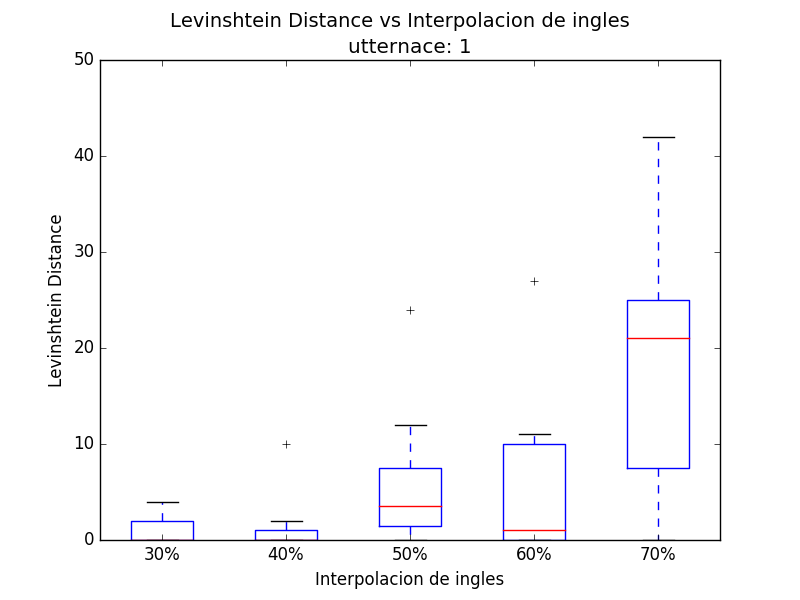
\includegraphics[width=.5\textwidth]{imagenes/plots_raw/1.png}&
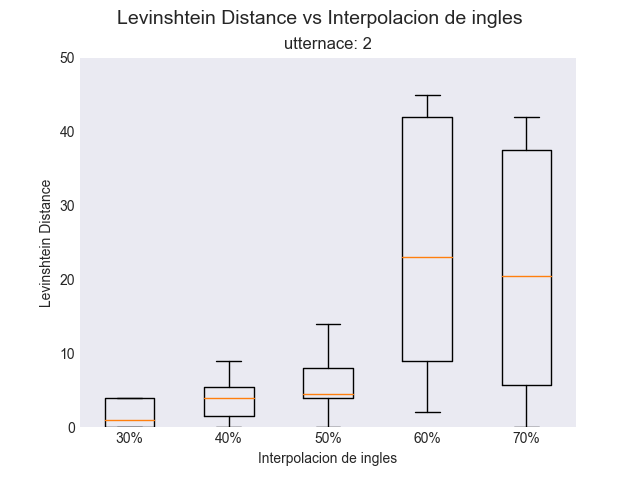
\includegraphics[width=.5\textwidth]{imagenes/plots_raw/2.png}
\end{array}$
\end{center}
\caption{Utternace 1 y 2}
\label{pics:blablabla}
\end{figure}

\clearpage

Como puede verse en la mayoría de los utternaces se puede observar que hasta el $50\%$ de mezcla castellano-ingles, se conserva el un buen grado de inteligibilidad, rondando la distancia de Levenshtein al rededor de $10$ a $20$ caracteres. Pasados el $60\%$ de ingles, se observa una disminución brusca en la inteligibilidad, llegando a una distancia de $45$ caracteres.

\begin{figure}[htp]
\begin{center}$
\begin{array}{lll}
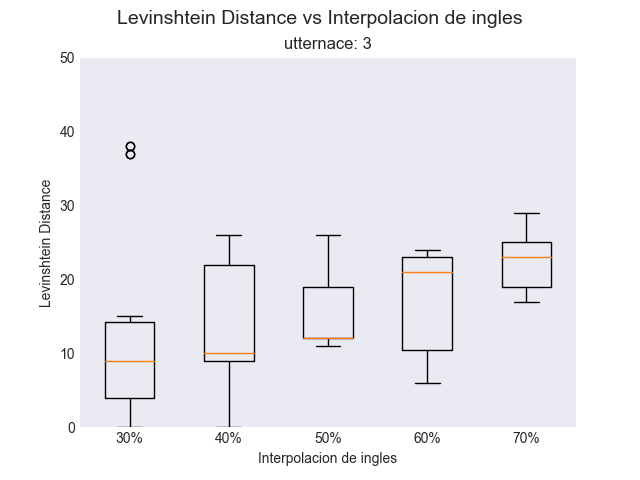
\includegraphics[width=.5\textwidth]{imagenes/plots_raw/3.png}&
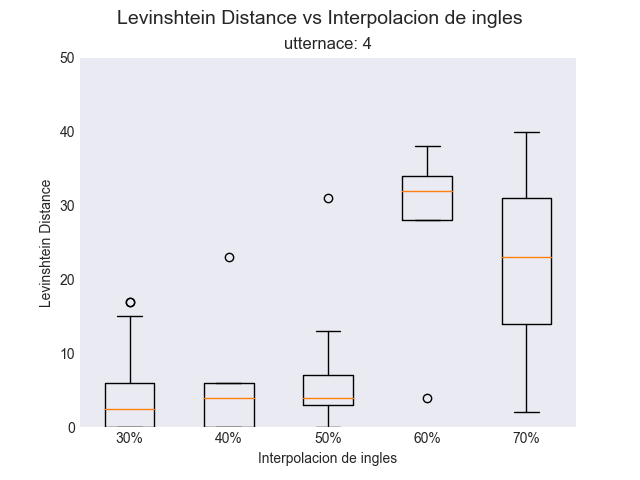
\includegraphics[width=.5\textwidth]{imagenes/plots_raw/4.png}
\end{array}$
\end{center}
\caption{Utternace 3 y 4}
\label{pics:blablabla}
\end{figure}
\clearpage

Analizando detenidamente las transcripciones obtenidas observamos algunas fallas sistemáticas que podrían generar ruido en el análisis, tales como:

\begin{itemize}
	\item Los participantes escribieron de manera diferente cuando no entendieron un segmento del audio.
		\begin{itemize}
		\item Muchos de ellos escribieron: ``...'', ``....'' o simplemente omitieron la palabra.
		\item En casos menos comunes: ``***'', ``???'', ``blablabla''.
		\end{itemize}
	\item En casos donde no comprendieron ninguna palabra del audio escribieron cosas como ``no entendí nada'', ``nada'', dejaron el campo vacío, etc.
	%\item Faltas ortografias del estilo: "grunion" en vez de "gruñón" que podría deberse a un teclado
	\item Utilización de signos de puntuación en las oraciones:
		\begin{itemize}
		\item Puntos finales para expresar el final de la oración o expresiones como ``(?)''.
		\item En un caso extremo, un participante el participante transcribió `` ``tu estrecho posavasos'', grito la fechoría'', cuando el Utternace original solo decía ``tu estrecho portavasos gritó la fechoría''.
		\end{itemize}
	\item Omisión de acentos y faltas ortográficas en palabras que no ambiguas.Ejemplo: ``grunion'' en vez de ``gruñón''
\end{itemize}

\begin{figure}[htp]
\begin{center}$
\begin{array}{lll}
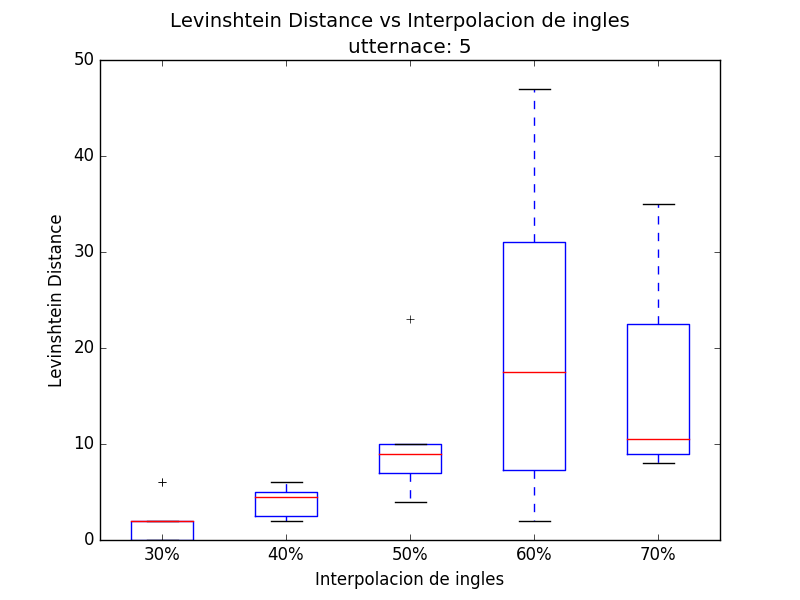
\includegraphics[width=.5\textwidth]{imagenes/plots_raw/5.png}&
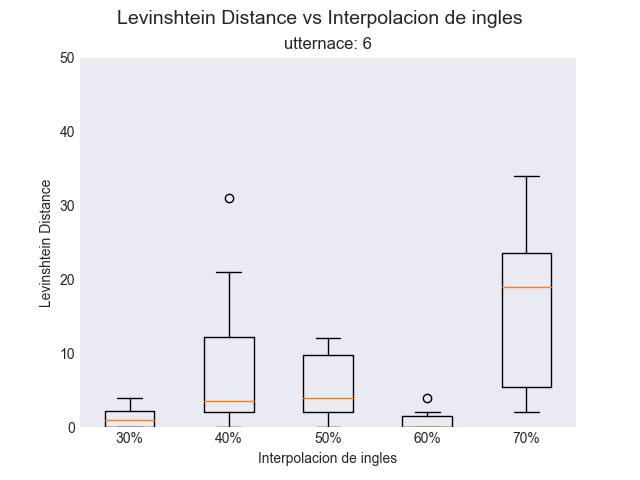
\includegraphics[width=.5\textwidth]{imagenes/plots_raw/6.png}
\end{array}$
\end{center}

\caption{Utternace 5 y 6}
\label{pics:blablabla}
\end{figure}

\begin{figure}[htp]
\begin{center}$
\begin{array}{lll}
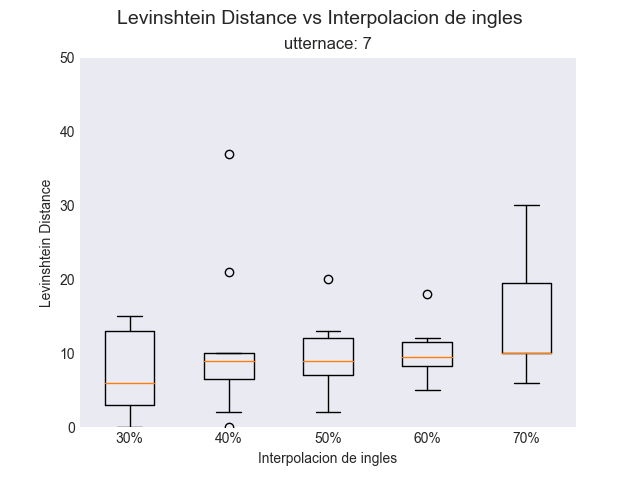
\includegraphics[width=.5\textwidth]{imagenes/plots_raw/7.png}&
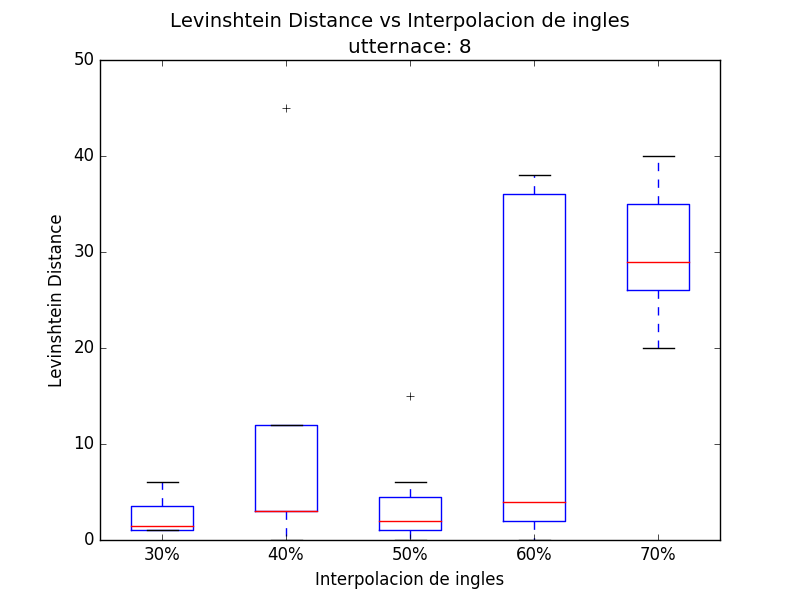
\includegraphics[width=.5\textwidth]{imagenes/plots_raw/8.png}
\end{array}$
\end{center}
\caption{Utternace 7 y 8}
\label{pics:blablabla}
\end{figure}

Para disminuir ruido de la muestra, se decidió realizar una limpieza de los datos donde consideramos que no era disruptiva.

Los cambios fueron:

\begin{itemize}
\item corregir ``ni'' por ``ñ '' en la palabra grunion.
\item Remoción de todos los signos de puntuación. 
\item Remoción de expresiones como ``blabla'', "no entendí" o cualquier otra que exprese ininteligibilidad de una palabra u oración.
\item Corrección de acentos en palabras no ambiguas: ``botón'', ``prefirió'', ``recorrió'', ``chupetín'', ``riñón'', ``gruñón''.
%otros ejemplos: apoyo, enfrío
\end{itemize}

Aquellas palabras que presentan ambivalencia, como : ``concluyó'' no fueron modificadas ya que concluyó/concluyo son validas.

\begin{figure}[htp]
\begin{center}$
\begin{array}{lll}
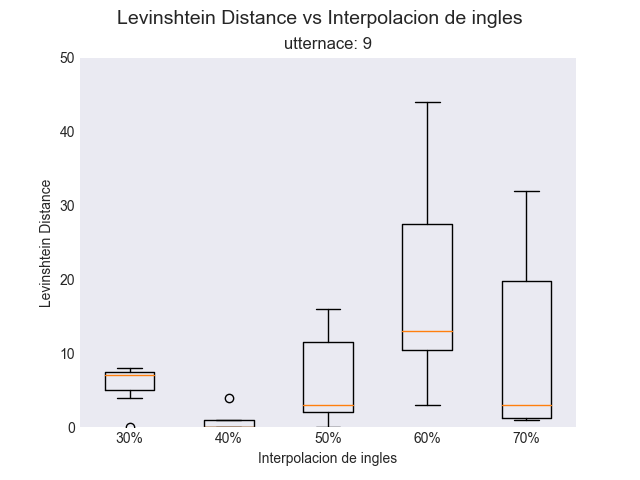
\includegraphics[width=.5\textwidth]{imagenes/plots_raw/9.png}\quad
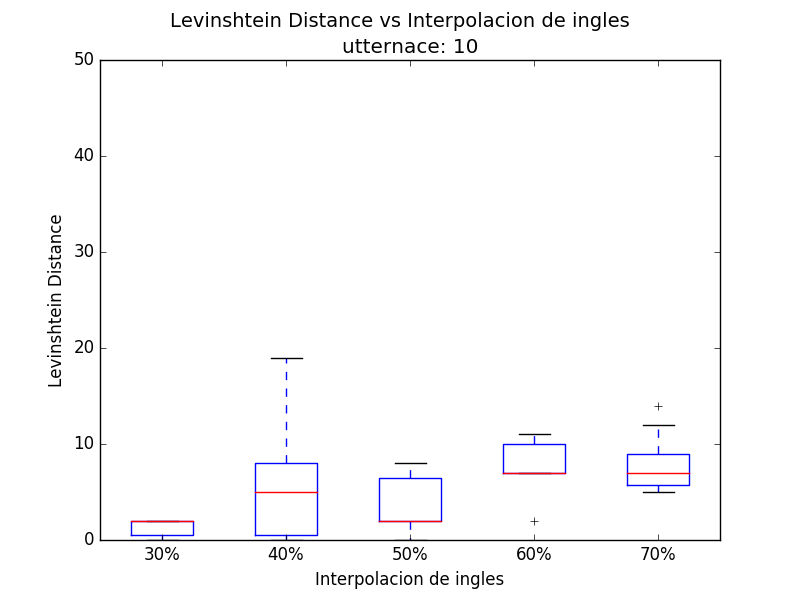
\includegraphics[width=.5\textwidth]{imagenes/plots_raw/10.png}
\end{array}$
\end{center}
\caption{Utternace 9 y 10}
\label{pics:blablabla}
\end{figure}


Esta normalización no solamente ayudará a disminuir la propagación de los datos sino que nos permitirá entender de manera mas intuitiva que significa la distancia de Levenshtein en cada caso.


\clearpage

\subsubsection{Datos normalizados}

Con esta estandarización de los datos, trataremos de darles un peso intuitivo que nos permitan sistematizar el análisis.

Por ejemplo, tomando el Utternace $8$ de las frases utilizadas en la experimentación: 

\begin{itemize}
	\item ``Las acongojadas cotorras sonrieron a mi círculo''
\end{itemize}

Podemos observar que:

\begin{itemize}
	\item Distancia 0: ``Las acongojadas cotorras sonrieron a mi círculo''
	\item Distancia 10: ``Las acontojadas culturas sonrieron en semicírculo''
	\item Distancia 20: ``Plaza sombreada con sombrero sonrieron en mi círculo''
	\item Distancia 30: ``sonrieron en mi círculo''
	\item Distancia 40: ``círculo''
	\item Distancia 48: ``''
\end{itemize}

A partir de esto, para este apartado vamos a tomar que una distancia de Levenshtein

\begin{itemize}
	\item Distancia 0-10: Buena Inteligibilidad
	\item Distancia 10-20: Mediana Inteligibilidad
	\item Distancia 20-40: Baja Inteligibilidad
	\item Distancia 40-: Inteligibilidad nula
\end{itemize}

\begin{figure}[htp]
\begin{center}$
\begin{array}{lll}
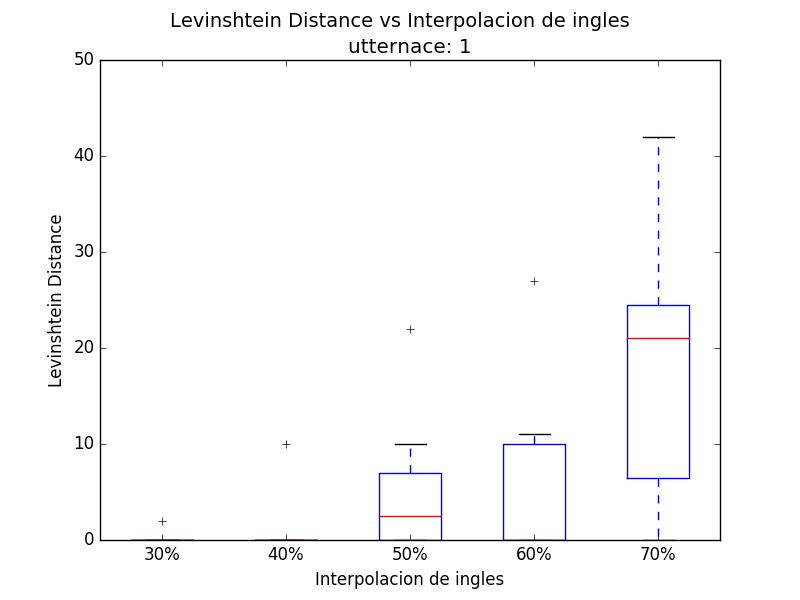
\includegraphics[width=.5\textwidth]{imagenes/plots_normalized/1.png}&
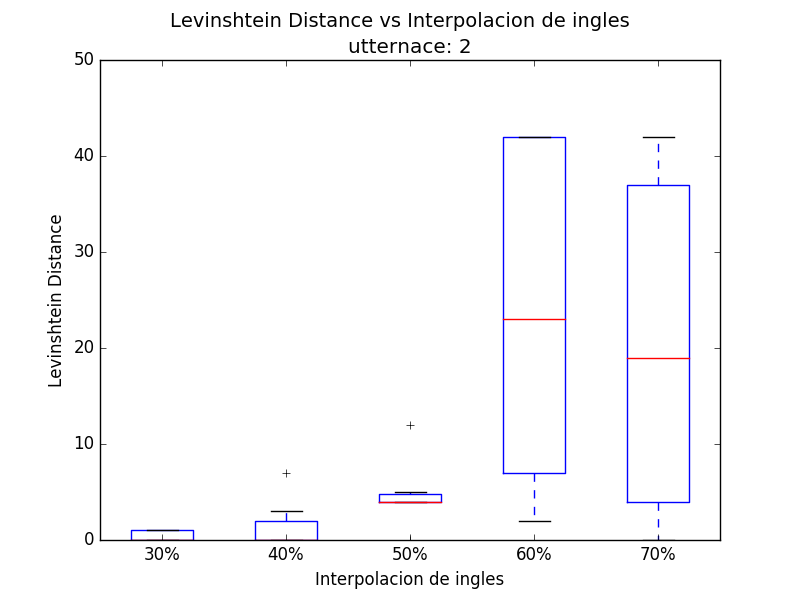
\includegraphics[width=.5\textwidth]{imagenes/plots_normalized/2.png}
\end{array}$
\end{center}
\caption{Utternace 1 y 2 Normalizados}
\label{pics:blablabla}
\end{figure}

Con este baseline, podemos ver que para una interpolación de ingles de $30\%$, $96$ de los $106$ participantes comprendieron de manera adecuada el texto con una inteligibilidad alta. Los $10$ restantes obtuvieron una inteligibilidad media. 

\begin{figure}[htp]
\begin{center}$
\begin{array}{lll}
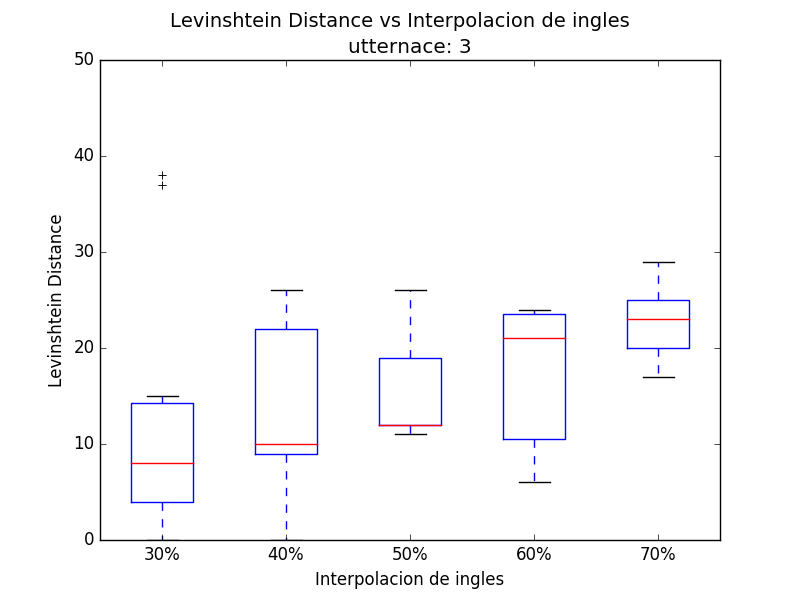
\includegraphics[width=.5\textwidth]{imagenes/plots_normalized/3.png}&
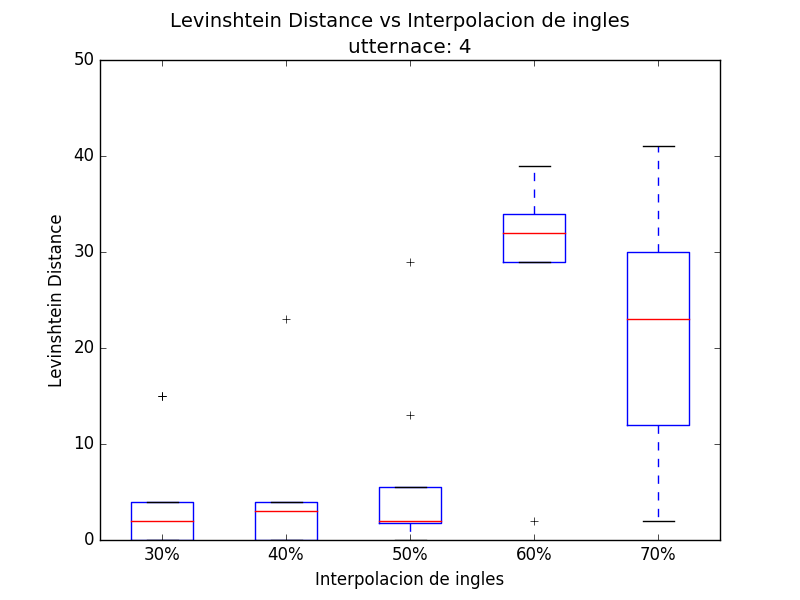
\includegraphics[width=.5\textwidth]{imagenes/plots_normalized/4.png}
\end{array}$
\end{center}
\caption{Utternace 3 y 4 Normalizados}
\label{pics:blablabla}
\end{figure}

Para la interpolación $40\%$ ingles - $60\%$ castellano, de un total de $67$ participantes, $57$ obtuvieron una inteligibilidad alta, $2$ una inteligibilidad media, $5$ una baja y 3 una inteligibilidad nula.


\begin{figure}[htp]
\begin{center}$
\begin{array}{lll}
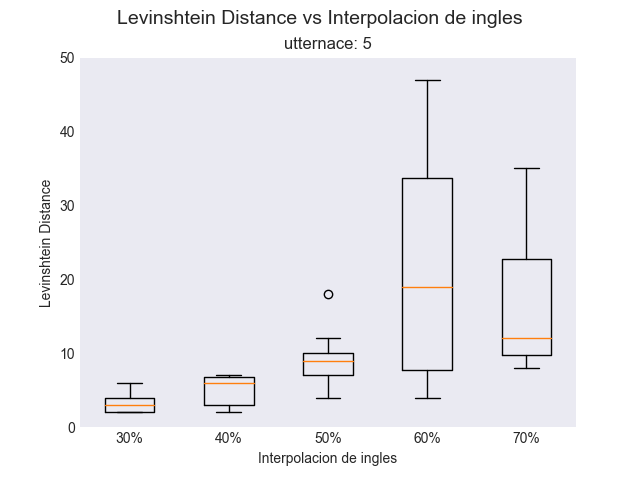
\includegraphics[width=.5\textwidth]{imagenes/plots_normalized/5.png}&
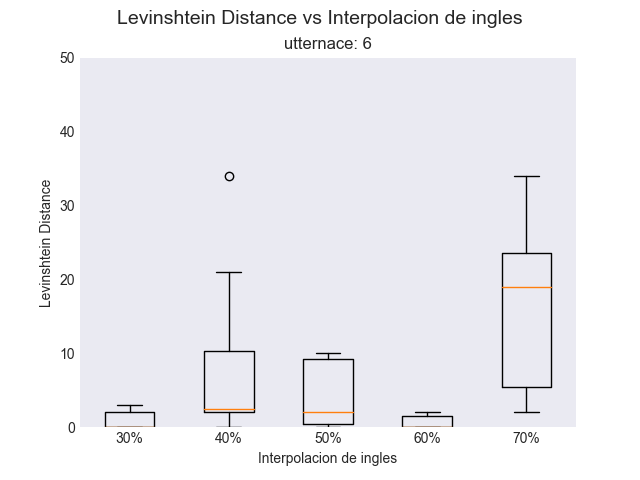
\includegraphics[width=.5\textwidth]{imagenes/plots_normalized/6.png}
\end{array}$
\end{center}
\caption{Utternace 5 y 6 Normalizados}
\label{pics:blablabla}
\end{figure}


Para la interpolación $50\%$ ingles - $50\%$ castellano, de un total de $75$ participantes, $57$ obtuvieron transcribir el audio demostrando una buena inteligibilidad, mientras que $14$ tuvieron una inteligibilidad media y $4$ una inteligibilidad baja.


Para todas las interpolaciones enunciadas previamente, los errores mas comunes varían desde falta de acentos en palabras como ``concluyó'' ambiguas hasta faltas de inteligibilidad en palabras con cierta complejidad como ``aguileña'' o ``gruñón''.


Para el Utternace $3$: ``este enjoyado juez comprará nuestro corchete'' observamos que la mayoría de los participantes cometieron errores al transcribir la palabra ``juez'' que confundieron de manera sistemática con palabras sonoramente similares como ``fue'', y ``enjoyado'' que transcribieron como ``enfollado'', ``enrollado'' y la conjugación exacta del verbo comprar.

\begin{figure}[htp]
\begin{center}$
\begin{array}{lll}
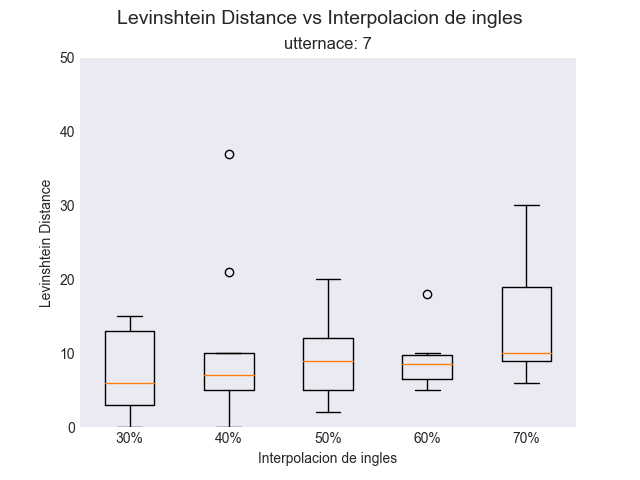
\includegraphics[width=.5\textwidth]{imagenes/plots_normalized/7.png}&
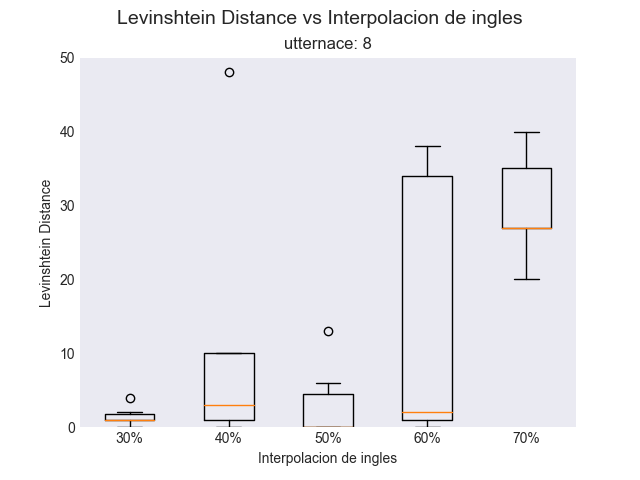
\includegraphics[width=.5\textwidth]{imagenes/plots_normalized/8.png}
\end{array}$
\end{center}
\caption{Utternace 7 y 8 Normalizados}
\label{pics:blablabla}
\end{figure}


Para los grados de interpolación $60\%$ ingles - $40\%$ castellano y $70\%$ ingles - $30\%$ castellano, se pueden observar un aumento notable de la variabilidad en las respuestas. Para el primero, de las $70$ respuestas obtenidas, $40$ participantes lograron transcribir con un buen grado de inteligibilidad los audios, $6$ obtuvieron una inteligibilidad media, y $24$ transcribieron el audio con una inteligibilidad baja o nula.


Para $70\%$ ingles - $30\%$ castellano, la diferencia es todavía mas marcada, de los $68$ resultados obtenidos, $28$ lograron transcribir el audio con un buen grado de inteligibilidad, $8$ con un grado medio y $32$ con un grado bajo o nulo de inteligibilidad.


\begin{figure}[htp]
\begin{center}$
\begin{array}{lll}
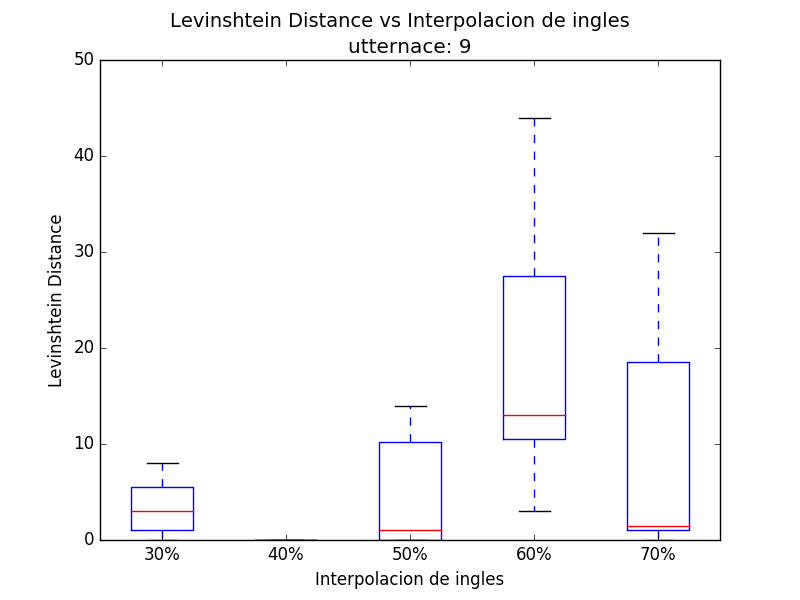
\includegraphics[width=.5\textwidth]{imagenes/plots_normalized/9.png}&
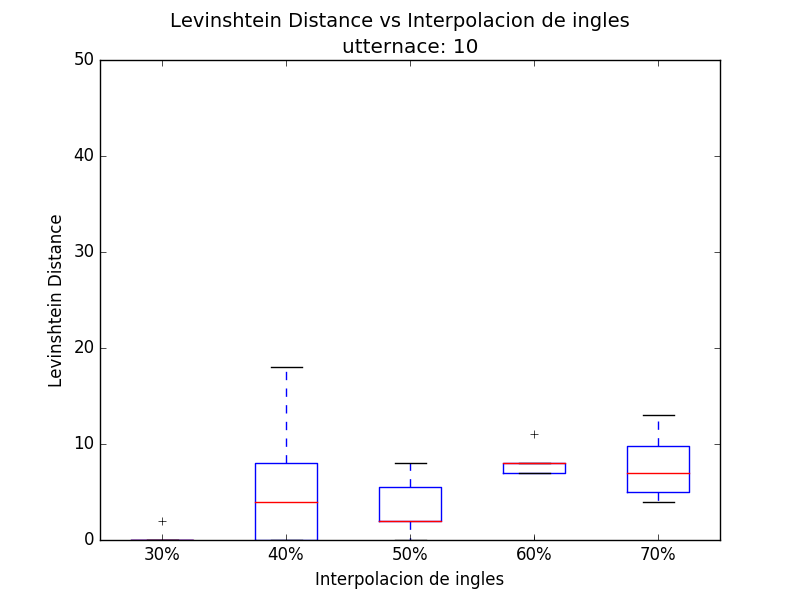
\includegraphics[width=.5\textwidth]{imagenes/plots_normalized/10.png}
\end{array}$
\end{center}
\caption{Utternace 9 y 10 Normalizados}
\label{pics:blablabla}
\end{figure}


Consideramos estos resultados tan dispares pueden deberse a dos motivos:


El primero, características particulares de los participantes y sus capacidades para discernir palabras incluso cuando presentan defectos en la pronunciación del hablante. En particular, el Utternace $4$ muestra como para un mismo audio, con características similares $2$ participantes de los 9 que realizaron la transcripción, obtuvieron distancias $2$ y $6$ en sus transcripciones.


El segundo motivo puede deberse a características particulares de los utternaces o del modelo utilizado para generar la voz: el Utternace $10$, donde el $6$ de los $8$ participantes obtuvieron una buena transcripción del audio, y el Utternace $8$, donde todos los participantes transcribieron el audio con inteligibilidad baja o nula, parecen demostrar esto. O bien la dificultad de los utternaces es variable o, lo que es todavía mas probable, llegado cierto punto en la interpolación, algunos fonemas empiezan a ``romperse'' o se alejan demasiado del fonema castellano correcto y terminan por disminuir la claridad de la voz.


%Agregar:
% python levinshteinFor.py 0
% Alta int: 96
% Media int: 10
% Baja int: 0
% nula: 4
% python levinshteinFor.py 1
% Alta int: 57
% Media int: 2
% Baja int: 5
% nula: 3
% porque nula? ver esto: parecen ser outliers
% python levinshteinFor.py 2
% Alta int: 57
% Media int: 14
% Baja int: 4
% nula: 0
% python levinshteinFor.py 3
% Alta int: 40
% Media int: 6
% Baja int: 11
% nula: 13
% python levinshteinFor.py 4
% Alta int: 28
% Media int: 8
% Baja int: 20
% nula: 12


\clearpage
\subsubsection{Análisis de Nacionalidad}


En esta sección analizaremos los resultados de las nacionalidades que los participantes atribuyeron a la voz.

Dado que en esta instancia se le le permitió a los participantes ingresar texto libre las respuestas resultaron bastante heterogéneas. Los participantes tomaron la consigna de manera diferente, pudiendo encontrarse respuestas que no pueden ser atribuidos exactamente a una nacionalidad. Ejemplo de algunas respuestas: Latino, Anglo, Robot, España (sur).

Consideramos que las respuestas de la índole ``robot'', ``es una voz artificial'', no son validas ya que no aportan información para esta investigación.

Por esta razón, en esta instancia decidimos agrupar las respuestas en cuatro grupos lógicos:

\begin{itemize}
	\item Hispanohablante: Latino, Argentino, Español, Uruguayo, Centroamericano, Boliviano, Mexicano, Colombiano
	\item Angloparlante: Estadounidense, Ingles, Irlandés, Canadiense, Anglo
	\item No sabe/No contesta: Robot, no se
	\item Otro: Ruso, Brasiltiño
\end{itemize}

Con estas agrupaciones, presentamos las nacionalidades atribuidas a la voz generada para cada punto de la interpolación.

\begin{figure}[htp]
\begin{center}$
\begin{array}{lll}
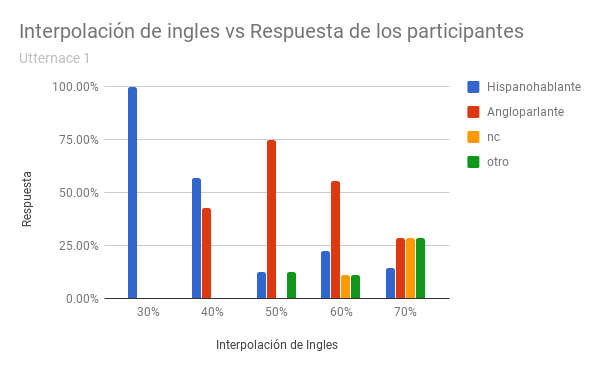
\includegraphics[width=.5\textwidth]{imagenes/nacionalidades/1.png}&
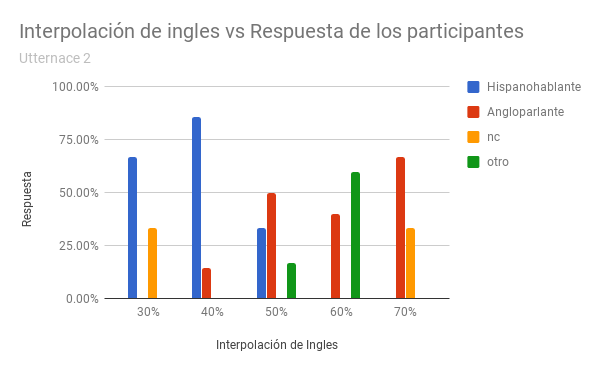
\includegraphics[width=.5\textwidth]{imagenes/nacionalidades/2.png}
\end{array}$
\end{center}
\caption{Utternace 1 y 2}
\label{pics:blablabla}
\end{figure}

De estos resultados podemos observar que con $30\%$ de interpolación de ingles, los participantes coinciden en que la voz puede atribuirse a una persona de habla nativa española.

\begin{figure}[htp]
\begin{center}$
\begin{array}{lll}
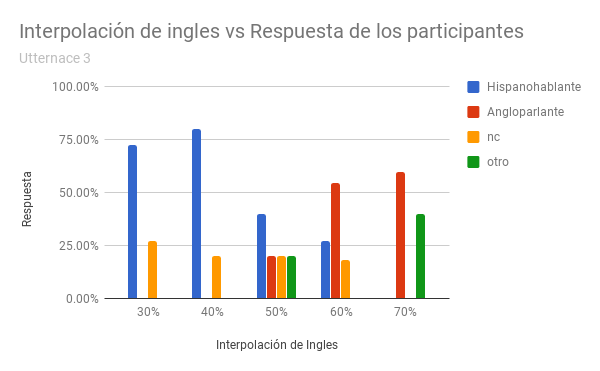
\includegraphics[width=.5\textwidth]{imagenes/nacionalidades/3.png}&
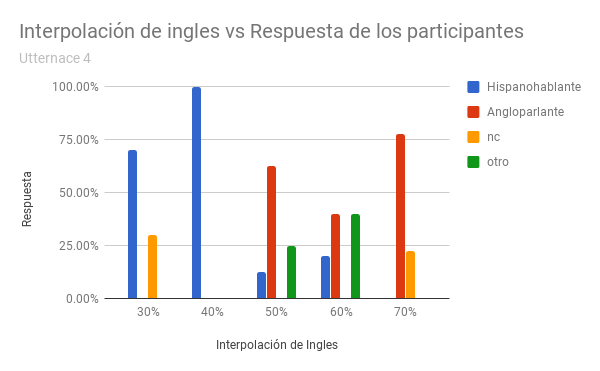
\includegraphics[width=.5\textwidth]{imagenes/nacionalidades/4.png}
\end{array}$
\end{center}
\caption{Utternace 3 y 4}
\label{pics:blablabla}
\end{figure}

Para una mezcla de $40\%$ ingles, puede verse que no hay una decisión concluyente con respecto a la nacionalidad del hablante. Por ejemplo en el Utternace 3 el $80\%$ de los participantes coincide que la voz pertenece a un hablante de habla hispana, mientras que en el Utternace 9 el $60.00\%$ de los participantes considera que la voz pertenece a un hablante de habla anglosajona.

Esta gran disparidad de resultados entre distintos utternaces se puede atribuir a las características particulares de cada Utternace. En particular el Utternace 9: ``Ese gruñón perro prometió a esos cuñados'' contiene una /r vibrante que resulta muy notoria al pronunciarse con una intensidad menor a la esperada y es atribuida, en general, a un hablante extranjero.
%perro vibrante múltiple alveolar sonora

Bajo esta suposición observamos que los otros utternaces que presentan este fonema:

\begin{itemize}
\item Utternace 1: ``Mi montaña aguileña recorrió la esquina'' 
\item Utternace 6: ``Su profundo riñón apoyó a Julio''
\item Utternace 7: ``El frío churrasco oyó lo de Polonia''
\item Utternace 8: ``Las acongojadas cotorras sonrieron a mi círculo''
\end{itemize}

También presentan un mayor porcentaje de atribuciones a nacionalidad anglosajona.

\begin{figure}[htp]
\begin{center}$
\begin{array}{lll}
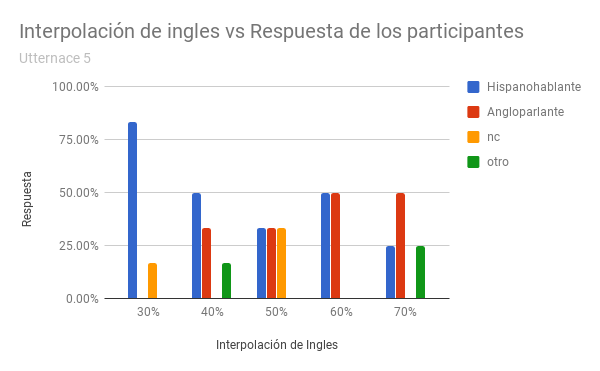
\includegraphics[width=.5\textwidth]{imagenes/nacionalidades/5.png}&
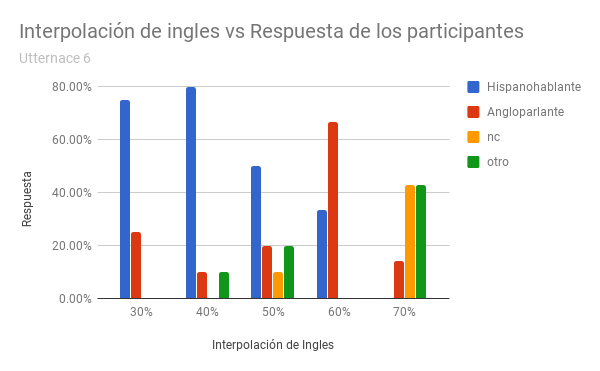
\includegraphics[width=.5\textwidth]{imagenes/nacionalidades/6.png}
\end{array}$
\end{center}
\caption{Utternace 5 y 6}
\label{pics:blablabla}
\end{figure}

Con $50\%$ y $60\%$ de ingles los resultados son similares. obtenemos que aproximadamente en el $50\%$ de los utternaces, mas de la mitad de los participantes consideraron que la voz pertenecía a un anglosajón hablando castellano. Para estos grados de interpolación también podemos observar que en un $80\%$ de los utternaces al menos un $20\%$ de los participantes atribuyen la nacionalidad del hablante a un no nativo no anglosajón hablando castellano.

\begin{figure}[htp]
\begin{center}$
\begin{array}{lll}
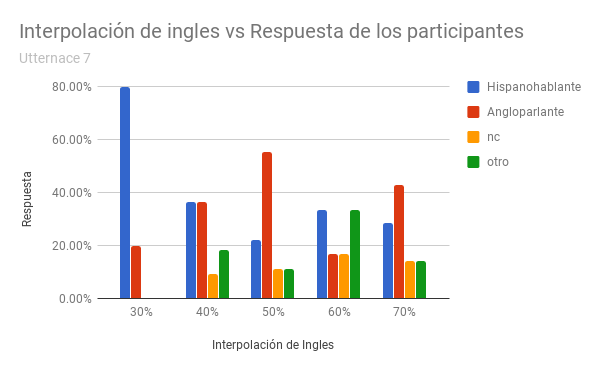
\includegraphics[width=.5\textwidth]{imagenes/nacionalidades/7.png}&
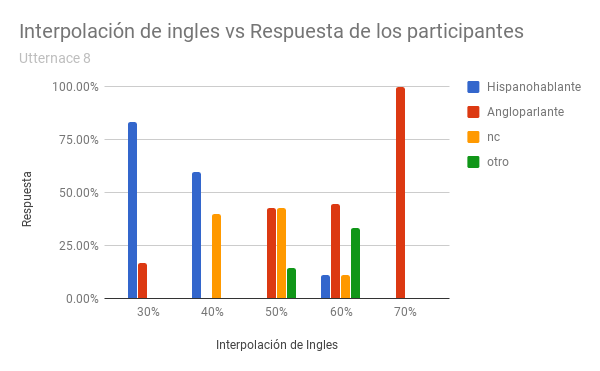
\includegraphics[width=.5\textwidth]{imagenes/nacionalidades/8.png}
\end{array}$
\end{center}
\caption{Utternace 7 y 8}
\label{pics:blablabla}
\end{figure}

Con $70\%$ de interpolación, en el $80\%$ de los utternaces se puede apreciar que al menos $50\%$ de los participantes dijo que el hablante era de origen anglosajón. Mas aún, en el $40\%$ de los utternaces el $75\%$ de los participantes coincidió que la voz era de angloparlante. También podemos ver que para este grado de interpolación en el $70\%$ de los utternaces ningún participante considera que la voz sea de habla hispana. En el $30\%$ restante, $25\%$ de los participantes o menos concideran que la voz pertenezca a un hispanohablante.

\begin{figure}[htp]
\begin{center}$
\begin{array}{lll}
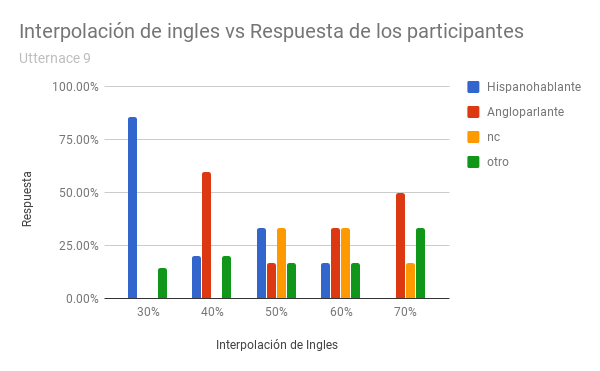
\includegraphics[width=.5\textwidth]{imagenes/nacionalidades/9.png}&
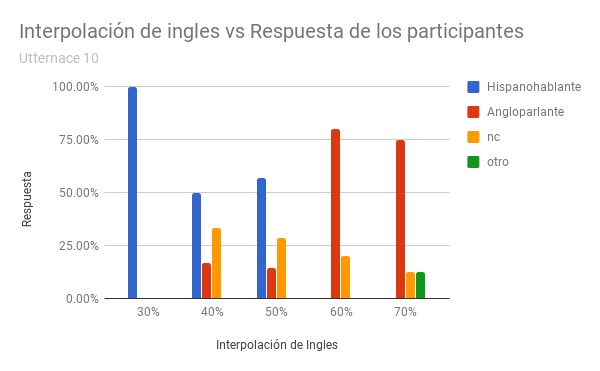
\includegraphics[width=.5\textwidth]{imagenes/nacionalidades/10.png}
\end{array}$
\end{center}
\caption{Utternace 9 y 10}
\label{pics:blablabla}
\end{figure}

%grafico general mostrando como crece el grado de ingles?

%conclucion mas general: aunque en muchos casos los participantes atribuyeron a la voz como un extrangero no anglosajon, tambien tener en cuenta que se esta intentando identificar la nacionalidad de un hablante con tan solo con una oración como referencia.

Hasta ahora analizamos los dos ejes de nuestra hipótesis por separado (por un lado, inteligibilidad, por otro, nacionalidad atribuida a la voz). En el ultimo apartado de la investigación buscaremos sacar conclusiones al componer ambos ejes en un mismo análisis.

\subsubsection{Resultados Generales de la experimentación}

Por ultimo visualizamos mostraremos la distancia de Levenshtein superpuesto con con la probabilidad de un participante de reconocer la voz como un hablante anglosajón.


\begin{figure}[htp]
\begin{center}$
\begin{array}{lll}
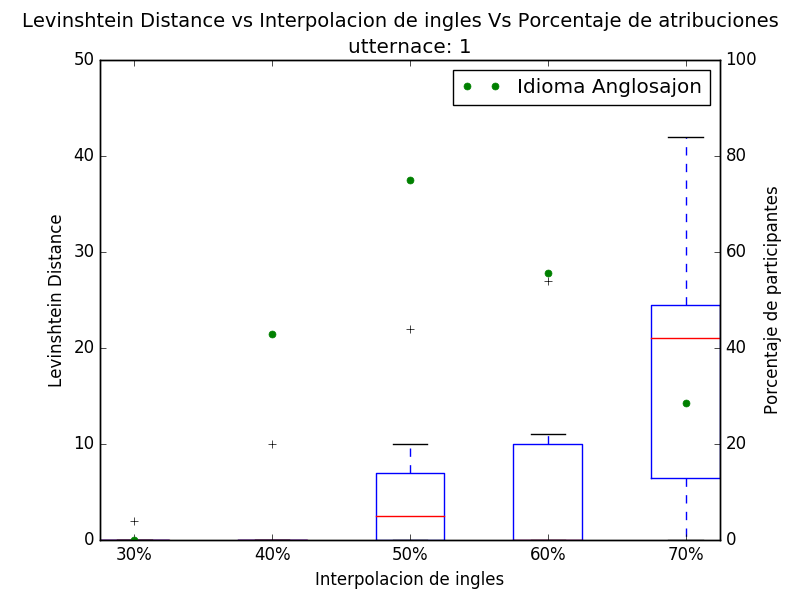
\includegraphics[width=.5\textwidth]{imagenes/nacVsPlot/1.png}&
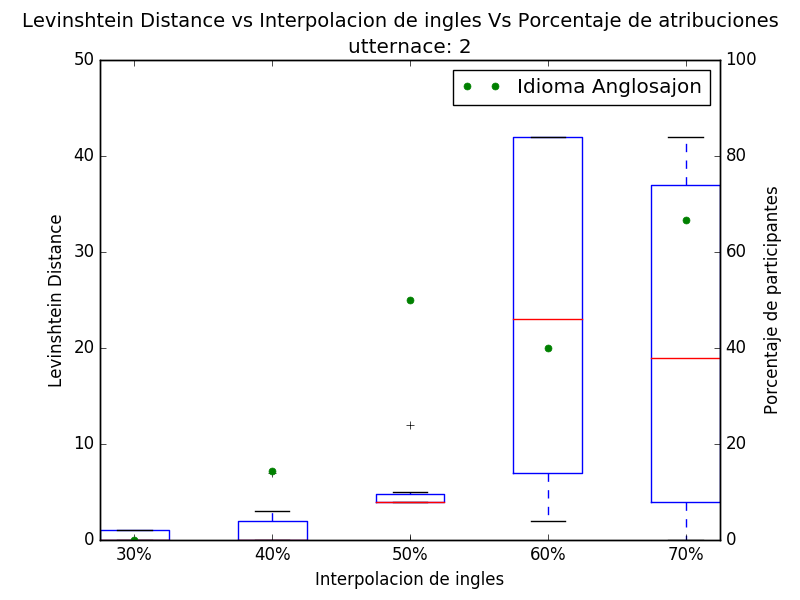
\includegraphics[width=.5\textwidth]{imagenes/nacVsPlot/2.png}
\end{array}$
\end{center}
\caption{Utternace 1 y 2}
\label{pics:blablabla}
\end{figure}


Volviendo a la hipótesis original, podemos ver que esta técnica permite generar una voz que pueda ser identificada como un extranjero hablando ingles, con un grado de efectividad que varía desde el $60\%$ hasta el $100\%$ dependiendo del Utternace elegido y el grado de interpolación.


\begin{figure}[htp]
\begin{center}$
\begin{array}{lll}
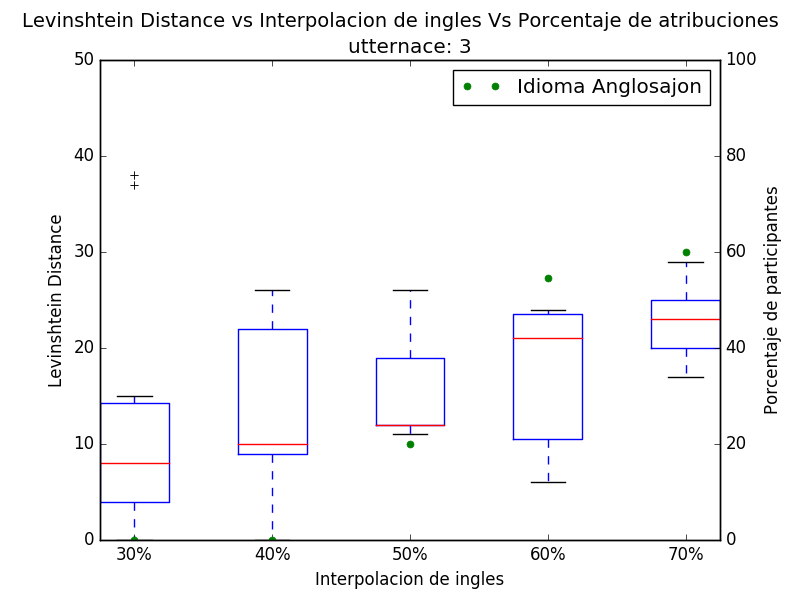
\includegraphics[width=.5\textwidth]{imagenes/nacVsPlot/3.png}&
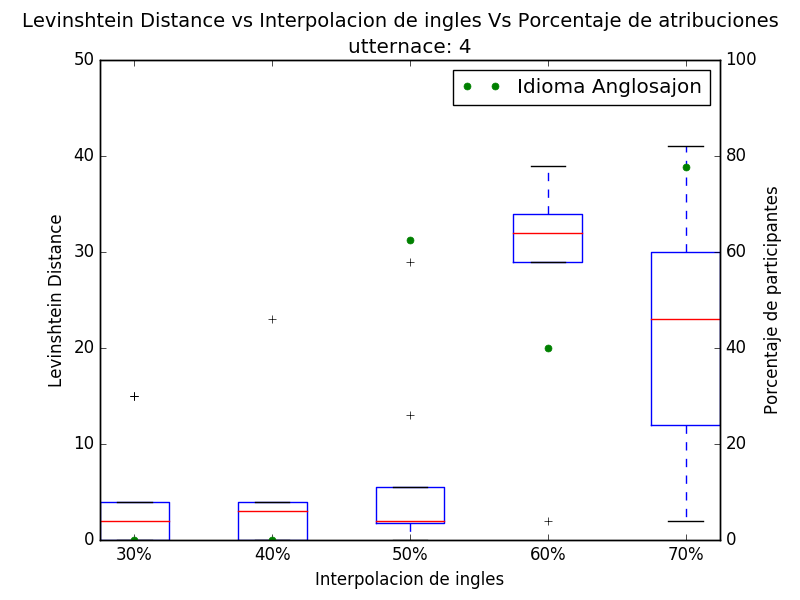
\includegraphics[width=.5\textwidth]{imagenes/nacVsPlot/4.png}
\end{array}$
\end{center}
\caption{Utternace 3 y 4}
\label{pics:blablabla}
\end{figure}


También es interesante observar casos como el que se presenta comparando el Utternace $10$ y el Utternace $8$, ambos con $70\%$ de mezcla de ingles, que en cuanto a inteligibilidad se encuentran en extremos opuestos, muestran que aproximadamente un $80\%$ y un $100\%$ de participantes identificaron como nativo anglosajón. Esto nos da a pensar que la inteligibilidad de una oración y su probabilidad de ser identificado como un hablante ingles son variables independientes y que este ultimo factor este mas ligado a otros factores como la sonoridad de ciertos fonemas o la prosodia general de la voz. 


Este no es un caso aislado, véase que lo mismo sucede con el Utternace $4$ y $6$ con $60\%$ de mezcla de ingles, si bien las inteligibilidades están en extremos opuestos, sus probabilidades de ser identificados como hablantes extranjeros difieren en menos del $20\%$.

\begin{figure}[htp]
\begin{center}$
\begin{array}{lll}
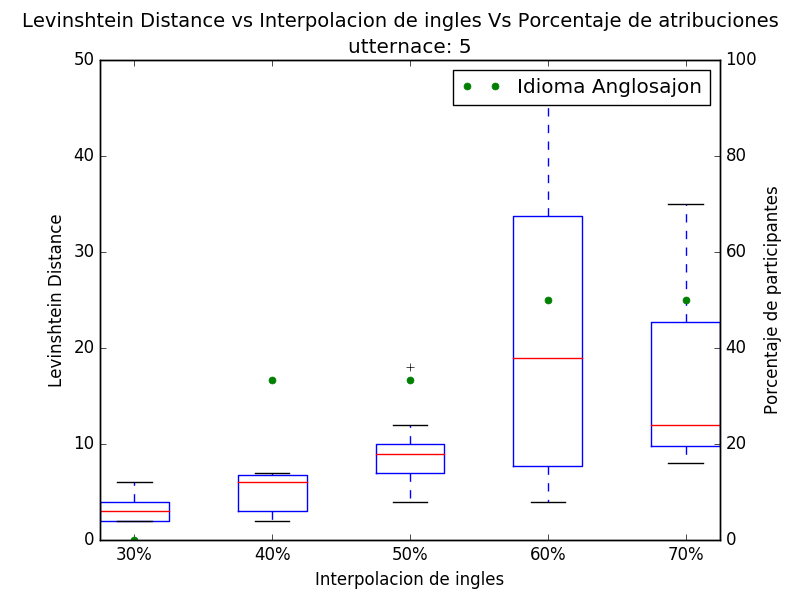
\includegraphics[width=.5\textwidth]{imagenes/nacVsPlot/5.png}&
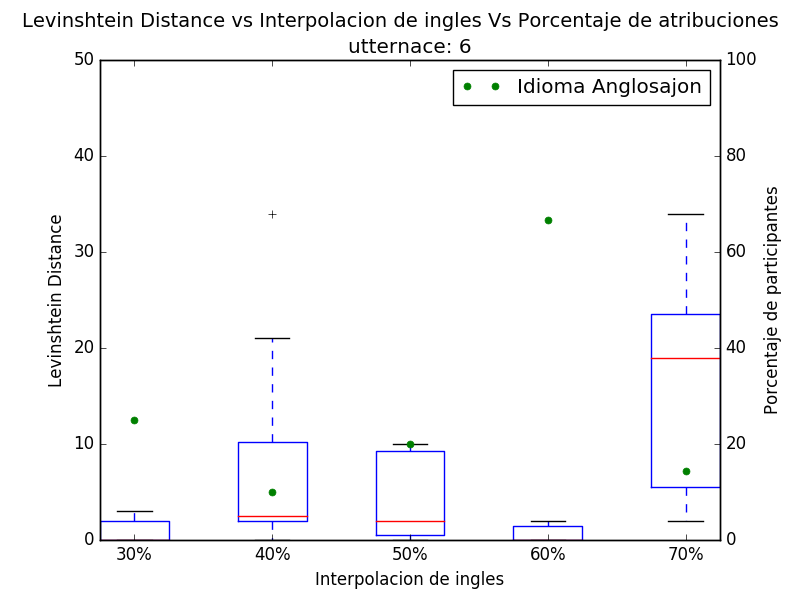
\includegraphics[width=.5\textwidth]{imagenes/nacVsPlot/6.png}
\end{array}$
\end{center}
\caption{Utternace 5 y 6}
\label{pics:blablabla}
\end{figure}

\begin{figure}[htp]
\begin{center}$
\begin{array}{lll}
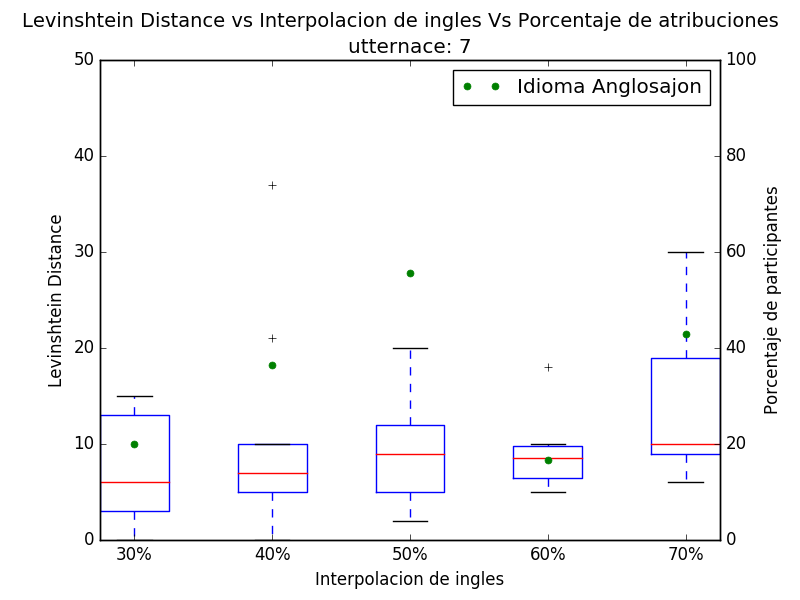
\includegraphics[width=.5\textwidth]{imagenes/nacVsPlot/7.png}&
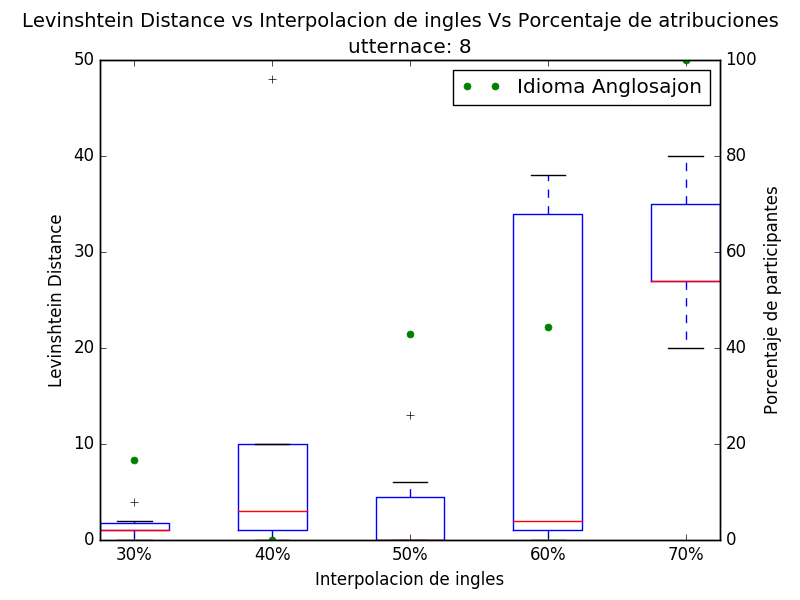
\includegraphics[width=.5\textwidth]{imagenes/nacVsPlot/8.png}
\end{array}$
\end{center}
\caption{Utternace 7 y 8}
\label{pics:blablabla}
\end{figure}

\begin{figure}[htp]
\begin{center}$
\begin{array}{lll}
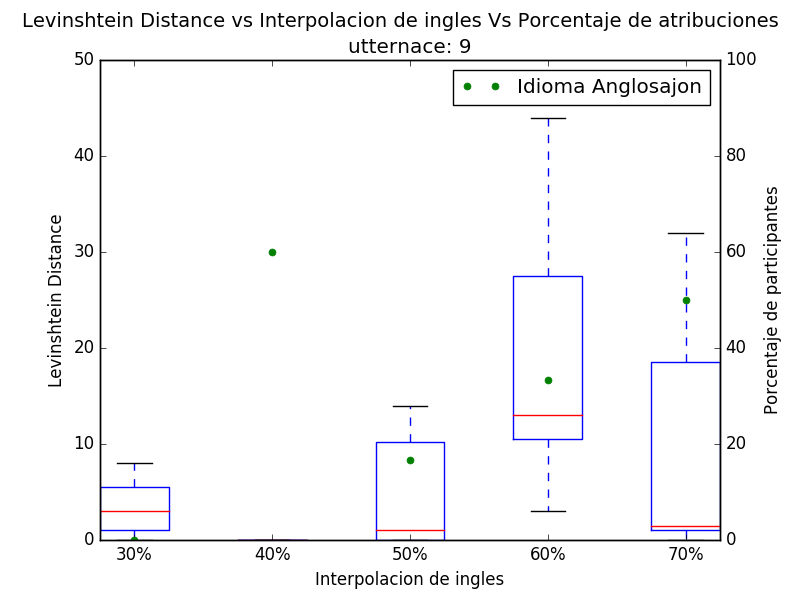
\includegraphics[width=.5\textwidth]{imagenes/nacVsPlot/9.png}&
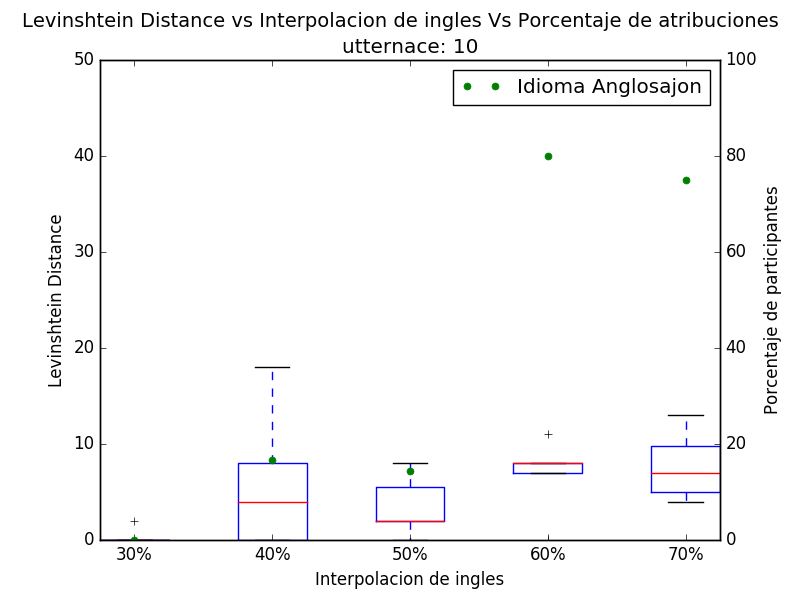
\includegraphics[width=.5\textwidth]{imagenes/nacVsPlot/10.png}
\end{array}$
\end{center}
\caption{Utternace 9 y 10}
\label{pics:blablabla}
\end{figure}




